% ############### 2.4) RUNTIME VIEW ####################

In order to make simpler diagrams, we decided to show only the main flow of the events, without considering all the possible alternatives and exceptions (every actor inserts the data correctly and satisfies their authorization requirements).
\newline
Additionally, we also note that the communication between the API gateway and the authorization server to generate the access token (to allow users to access only the resources they have permission for) has been left implicit.


\begin{figure}[H]
	\centering
    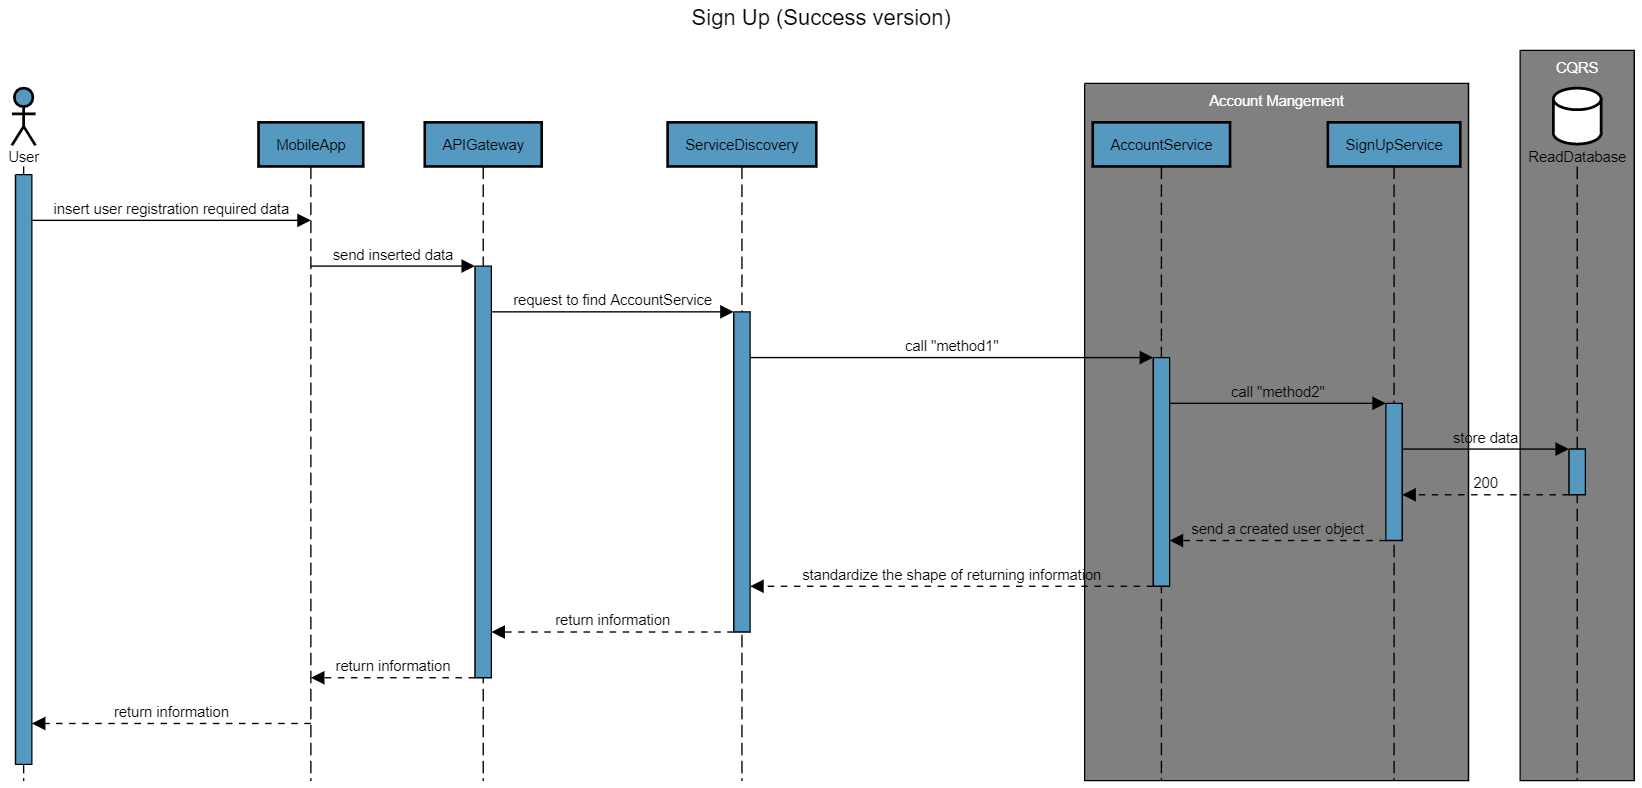
\includegraphics[width=\textwidth]{Images/sequence-diagram/sign-up.png}
	\caption{\label{fig:se_sign_up}Sign Up}
\end{figure}
Actor: All type of user


UI flow: {\ref{sec:user_mobile_interface} Sign Up, Login}
\newline
\newline
Firstly, this diagram explains the flow of sign up for all type of user. 
Due to CQRS pattern, there are two different database according to their purpose (\ref{sec:component_view}). 
\newline
\newline
\textsc{\textcolor{blue}{flow overview}}
\newline
Mobile App sends a method ”postUser()” to Mobile API Gateway, then service discovery finds a routing path by URL of REST API.
Then SignUpService receives post request. After that, to update the database, it sends command to Command handler to insert the data into Command DB, since it is a write operation.

\newpage
\begin{figure}[H]
	\centering
    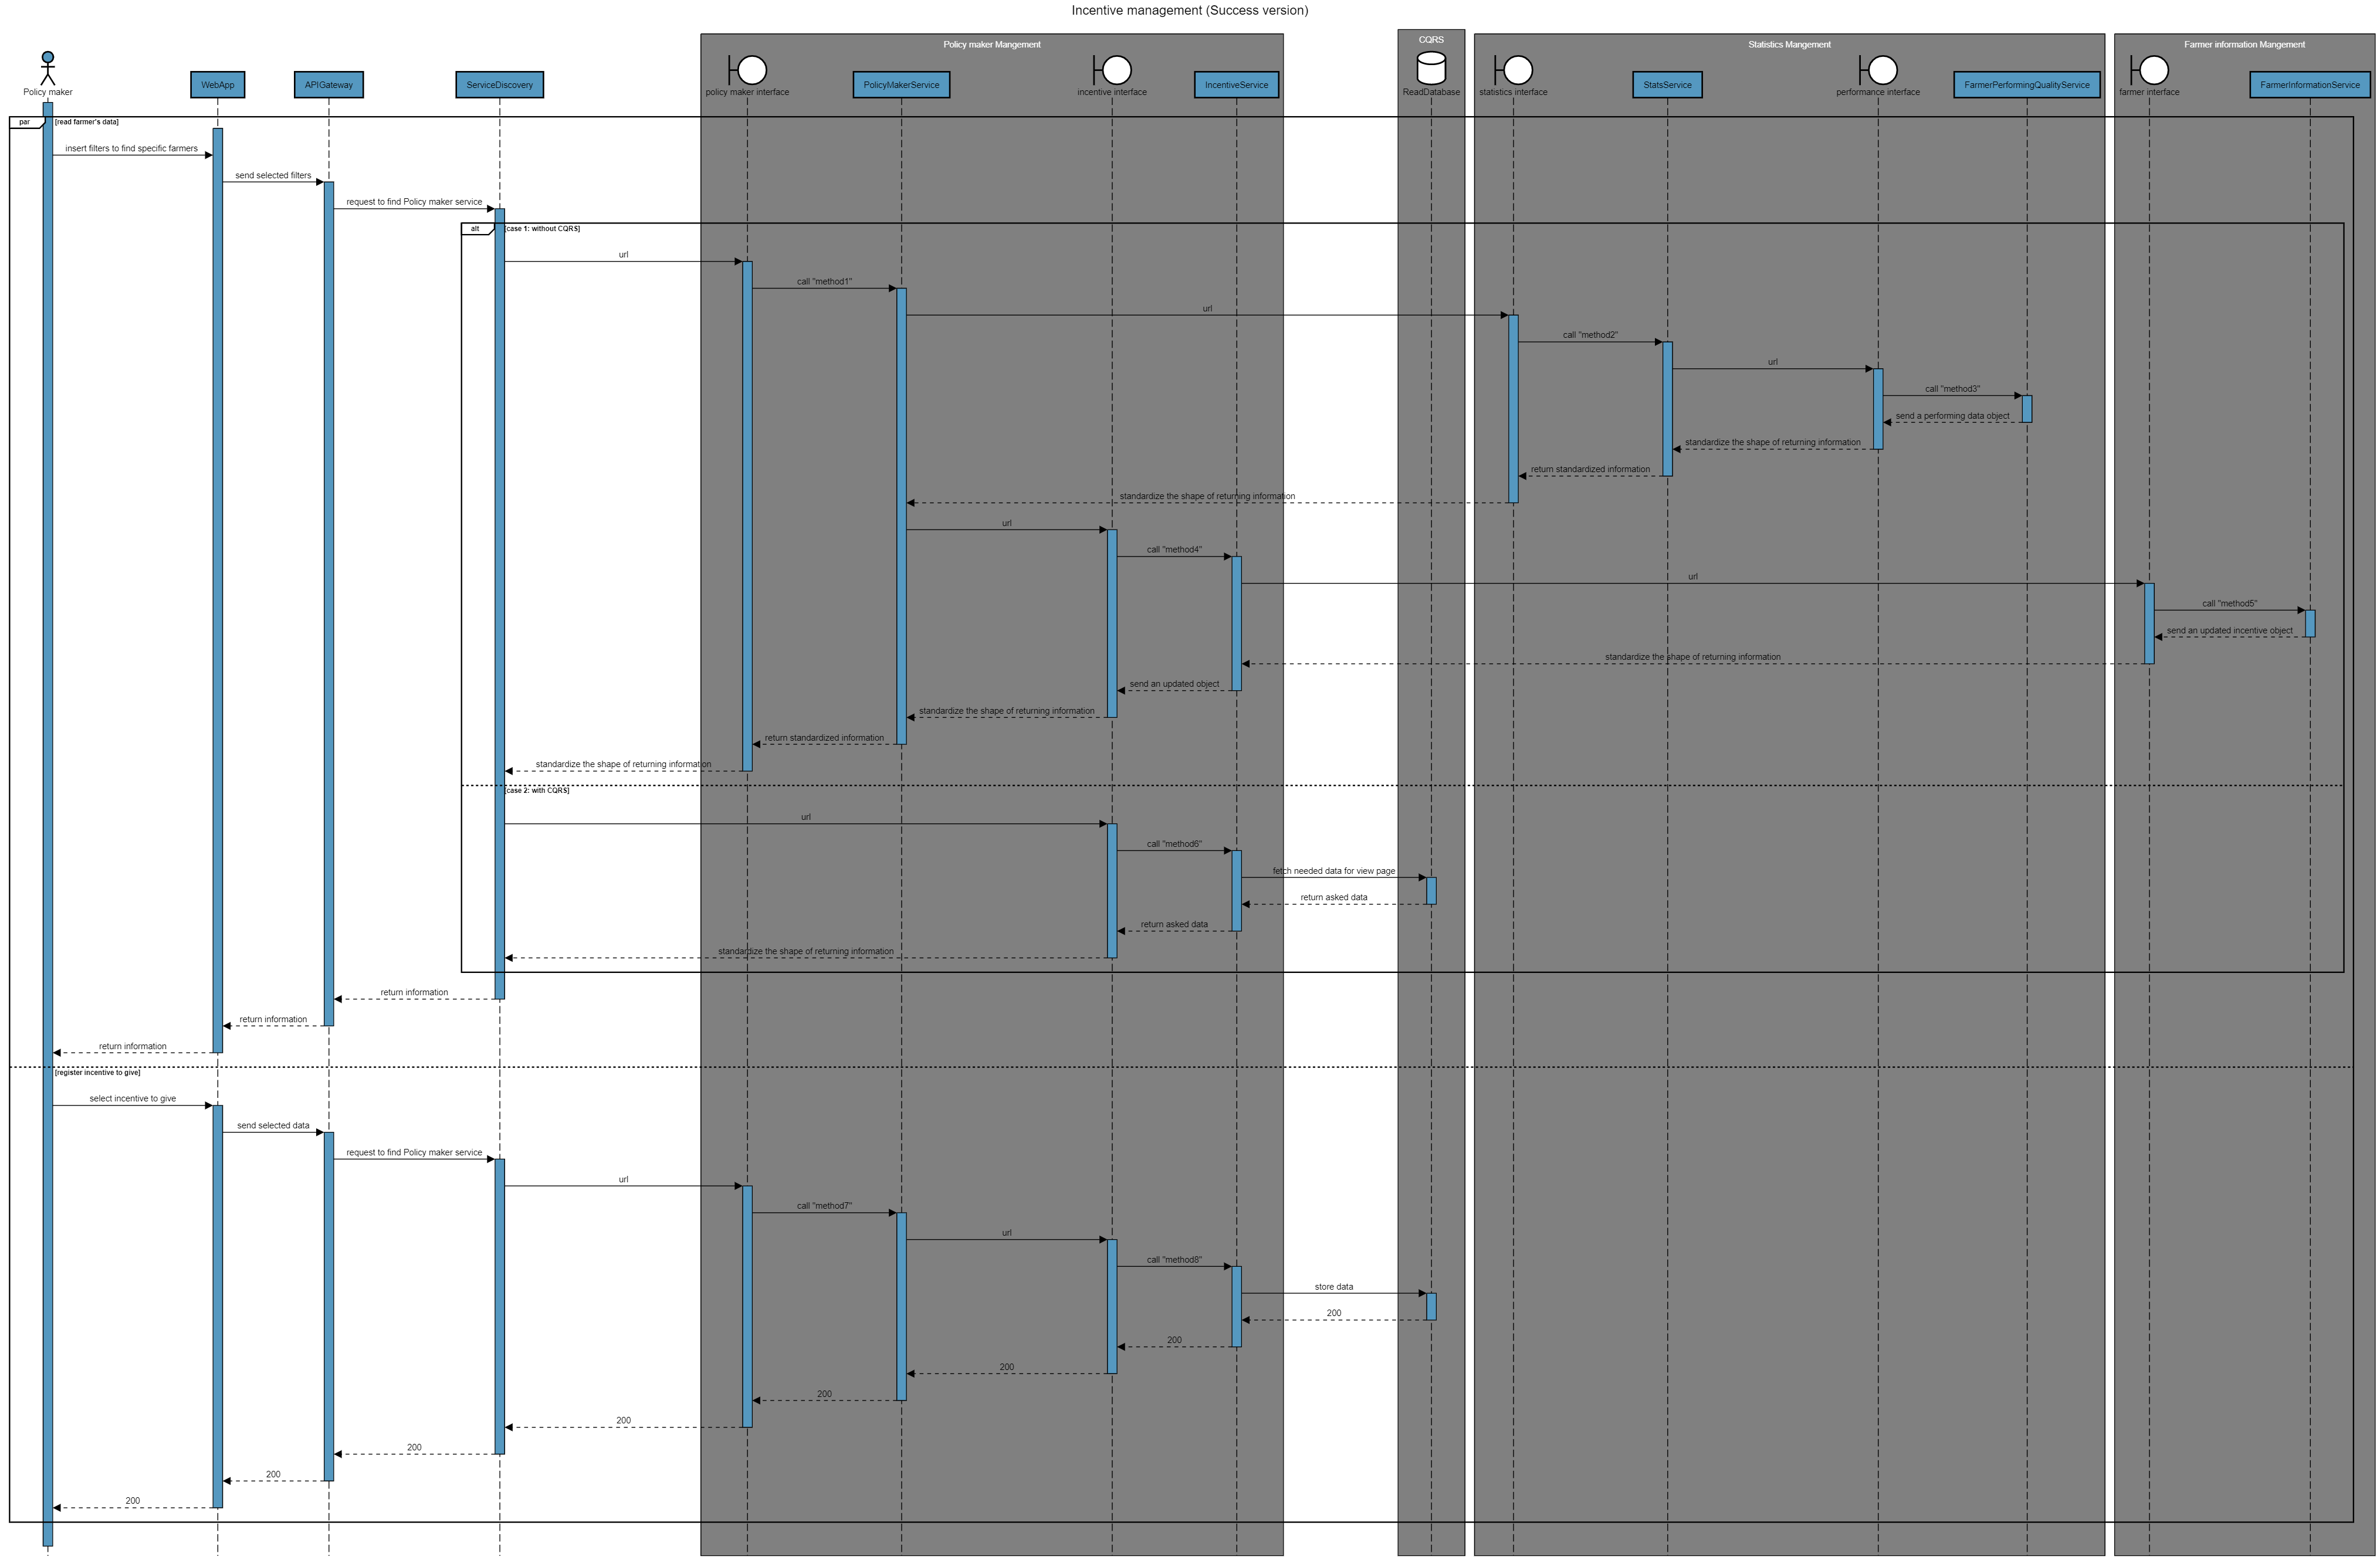
\includegraphics[width=\textwidth]{Images/sequence-diagram/incentive-management.png}
	\caption{\label{fig:se_incentive}Incentive management}
\end{figure}
Actor: Policy maker

UI flow: {\ref{sec:pm_web_interface} Farmer's performance data}
\newline
\newline
Secondly, we would like to highlight the reasoning of our design decision about this diagram. In the upper sequence flow we display how the interactions would be without the CQRS pattern, while in the lower flow we show the interactions with the CQRS pattern.
For the first part, by the fact we consider the analysis taken cared by 3rd party systems, it is also suitable to have replica of database to fetch aggregated data when it is needed, regardless of condition of their system.
\newline
\newline
\textsc{\textcolor{blue}{flow overview}}
\newline
Above part describes the flow of read operation: search and collect the data from the database. It is required to access Query DB.
Then, the below part explains the flow of write operation.
Incentive service needs to call Notification service to let the selected farmer receive it.

\newpage
\begin{figure}[H]
	\centering
    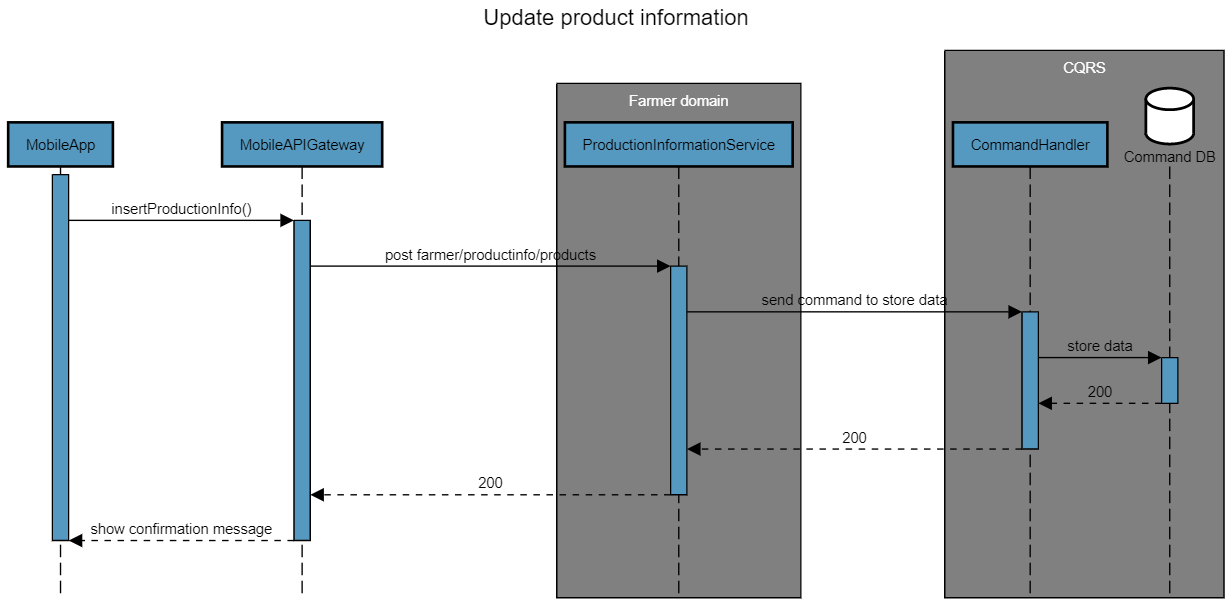
\includegraphics[width=\textwidth]{Images/sequence-diagram/product-info.png}
	\caption{\label{fig:se_product}Product information registration}
\end{figure}
Actor: Farmer

UI flow: {\ref{sec:farmer_mob_interface} Production data registration, Help/Suggestion request}
\newline
\newline
From now on, we consider that the communication between the API gateway and the discovery service, in order to find the exact service location, is implicit inside the API Gateway instance. Moreover, the interface of each microservice is no longer explicitly put in the diagram, to avoid redundant and less relevant information.
\newline
\newline
\textsc{\textcolor{blue}{flow overview}}
\newline
Farmer inserts needed information and sends the production data to register it. API gateway contacts to authorization server to assure the permission; if it is verified, then discovery service finds ProductInformationService and executes the method. Since it is a write operation, it sends data to Command handler to insert it into Command DB.

\newpage
\begin{figure}[H]
	\centering
    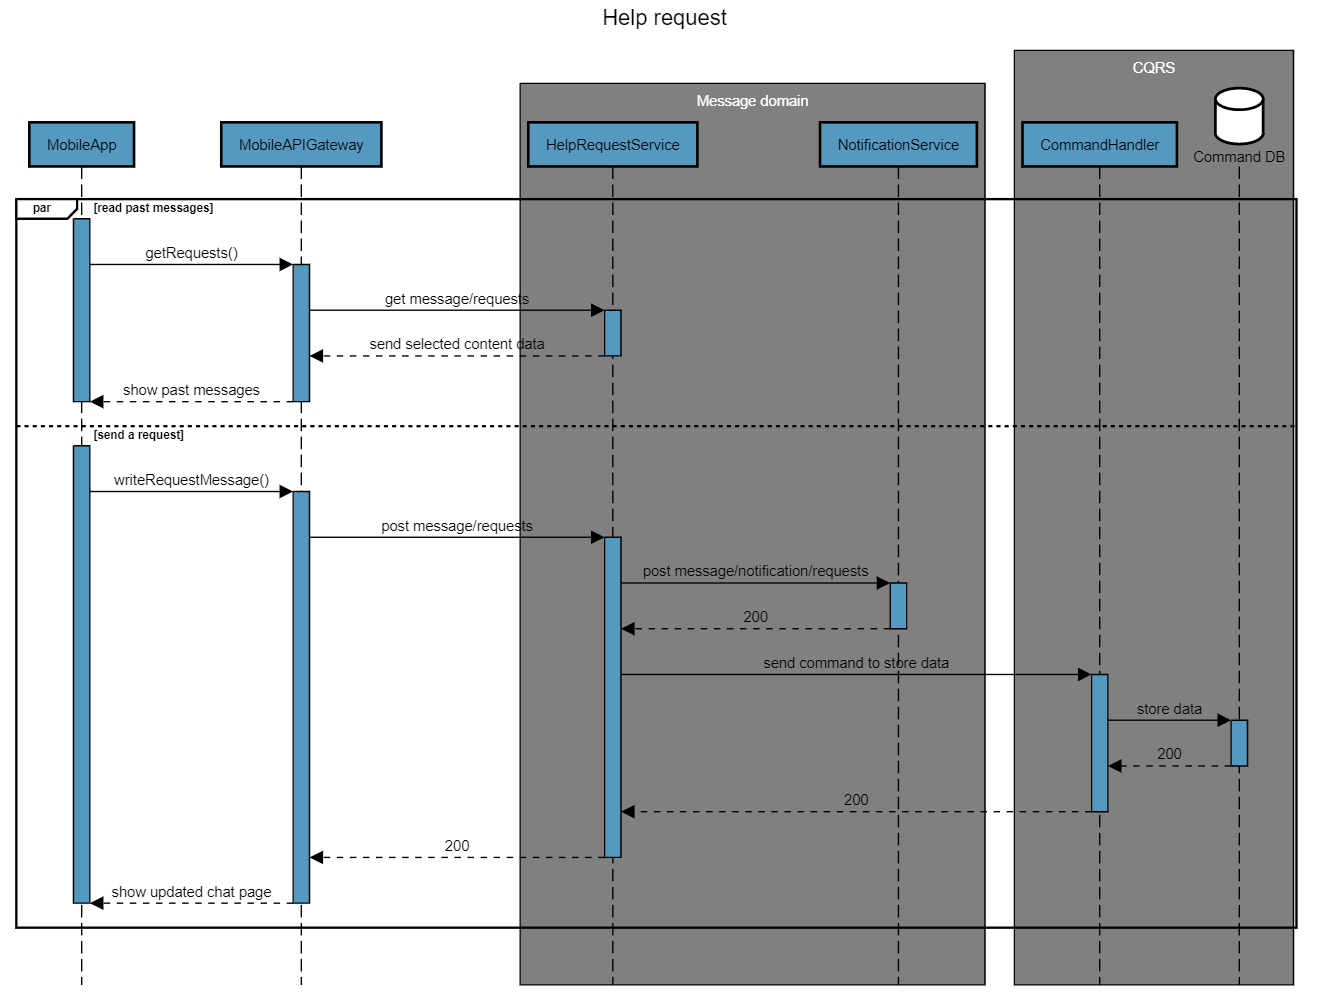
\includegraphics[width=\textwidth]{Images/sequence-diagram/help-request.png}
	\caption{\label{fig:se_help}Help request registration}
\end{figure}
Actor: Farmer

UI flow: {\ref{sec:farmer_mob_interface} Production data registration, Help/Suggestion request}
\newline
\newline
This diagram explains the flow of asking help request.
As a previous step, it requires the farmer to select whom they would like to ask the request, though we assumed this operation has been done in advance and the diagram above describes the phase afterwards.
\newline
\newline
\textsc{\textcolor{blue}{flow overview}}
\newline
First half shows the flow of read operation to visualize the past messages; on the other hand, the below part represents the write operation to send the message. 
For read operation, it does not access to Query DB since the data is not aggregated data, but it simply accesses the database inside of its own service.

\newpage
\begin{figure}[H]
	\centering
    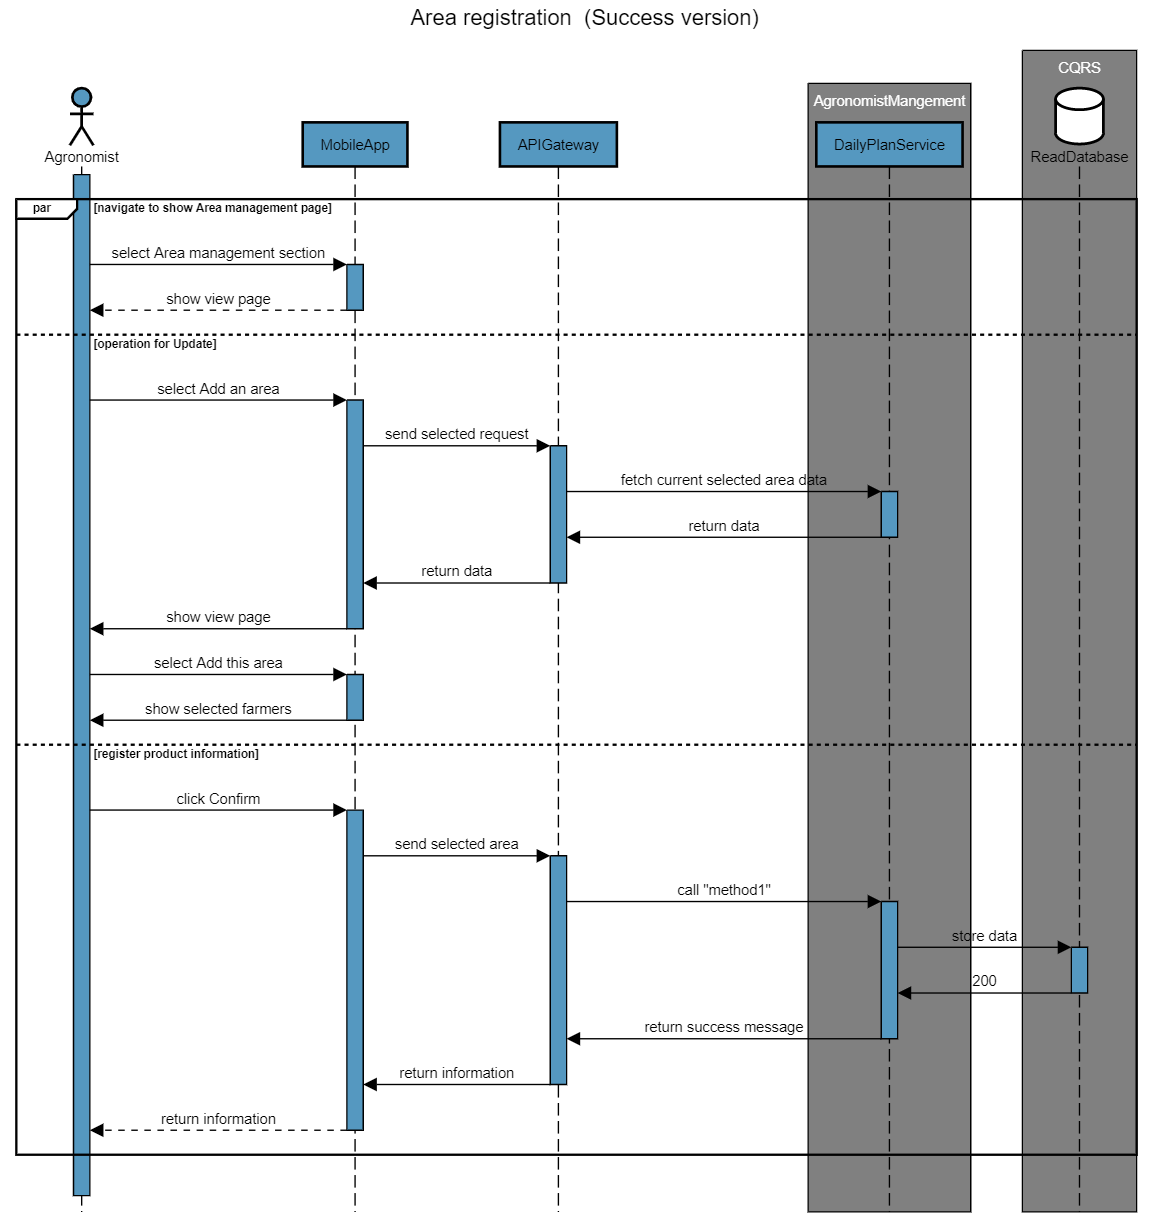
\includegraphics[width=\textwidth]{Images/sequence-diagram/area-registration.png}
	\caption{\label{fig:se_area}Area registration}
\end{figure}
Actor: Agronomist

UI flow: {\ref{sec:agronomist_mob_interface} Area management}
\newline
\newline
This diagram shows the flow of registering a new area to supervise. As like other examples, this diagram contains read and write operation individually.
\newline
\newline
\textsc{\textcolor{blue}{flow overview}}
\newline
Firstly, by calling getAreas(), the system will fetch current area information about the place (name of farmers, agronomists, ...). After the agronomists have observed area information, if they are interested in, they could register a new area to supervise. Write operation requires updating Command DB to let new registered data be reachable by other services.

\newpage
\begin{figure}[H]
	\centering
    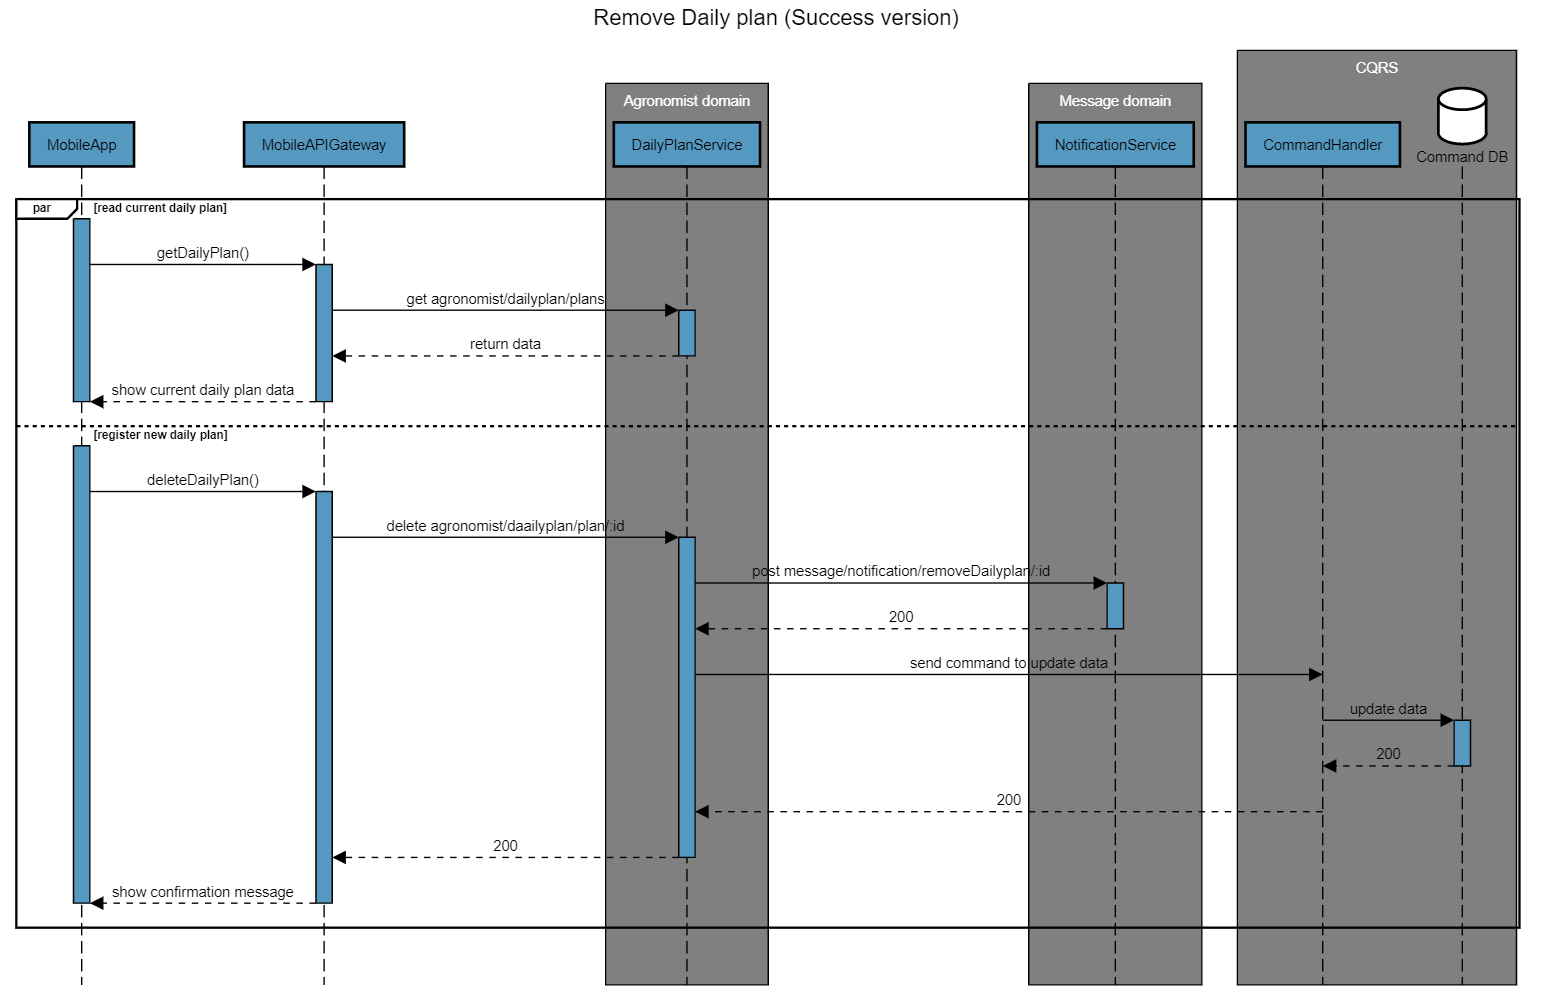
\includegraphics[width=\textwidth]{Images/sequence-diagram/daily-plan.png}
	\caption{\label{fig:se_daily}Remove Daily plan}
\end{figure}
Actor: Agronomist

UI flow: {\ref{sec:agronomist_mob_interface} Daily plan management}
\newline
\newline
As the last example, this diagram shows the flow of updating daily plan of agronomist.
Unlike other insertion examples, here it deletes the record from database, so it requires DELETE method.
\newline
\newline
\textsc{\textcolor{blue}{flow overview}}
\newline
On the upper part, the system lets agronomists know the daily plan they have. Instead, the bottom part explains the flow of deletion operation. By specifying the ID in the URL, Command Handler searches the record that owns that id and deletes it.